\section{Detalji penjačke lokacije}

\begin{figure}[H]
    \centering
    \begin{subfigure}[b]{\textwidth}
        \centering
        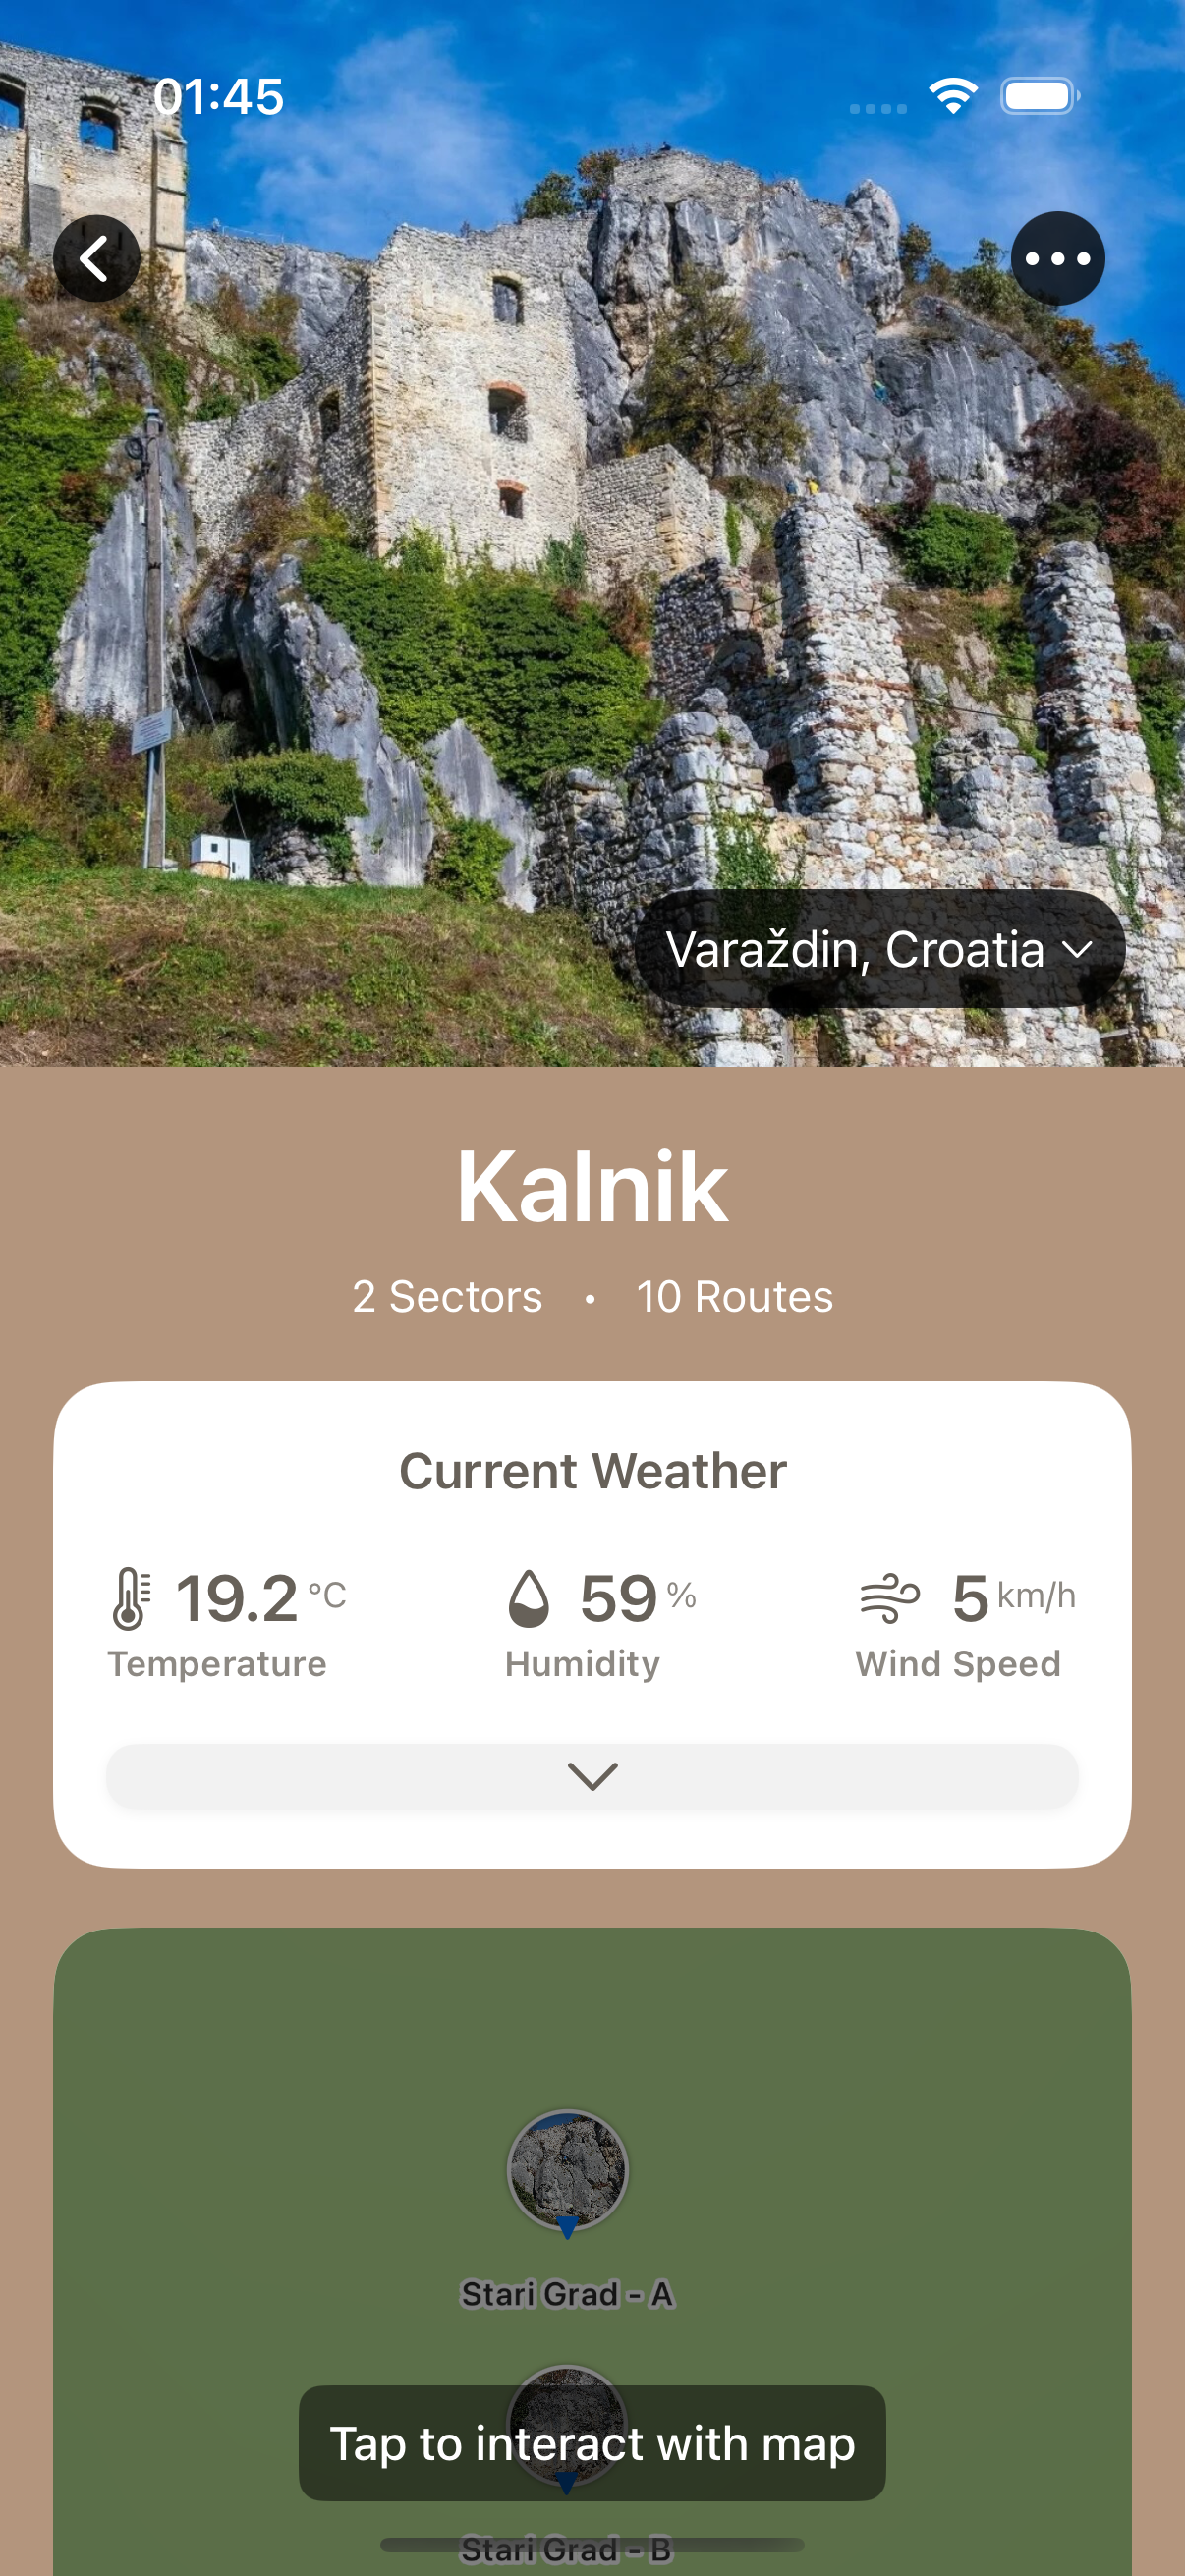
\includegraphics[width=0.3\textwidth]{images/implementacija/crag-details/crag-details-top.png}
        \caption{Mobilna aplikacija}
        \label{fig:detalji_penjackih_lokacija_mob}
    \end{subfigure}
    \hfill
    \begin{subfigure}[b]{\textwidth}
        \centering
        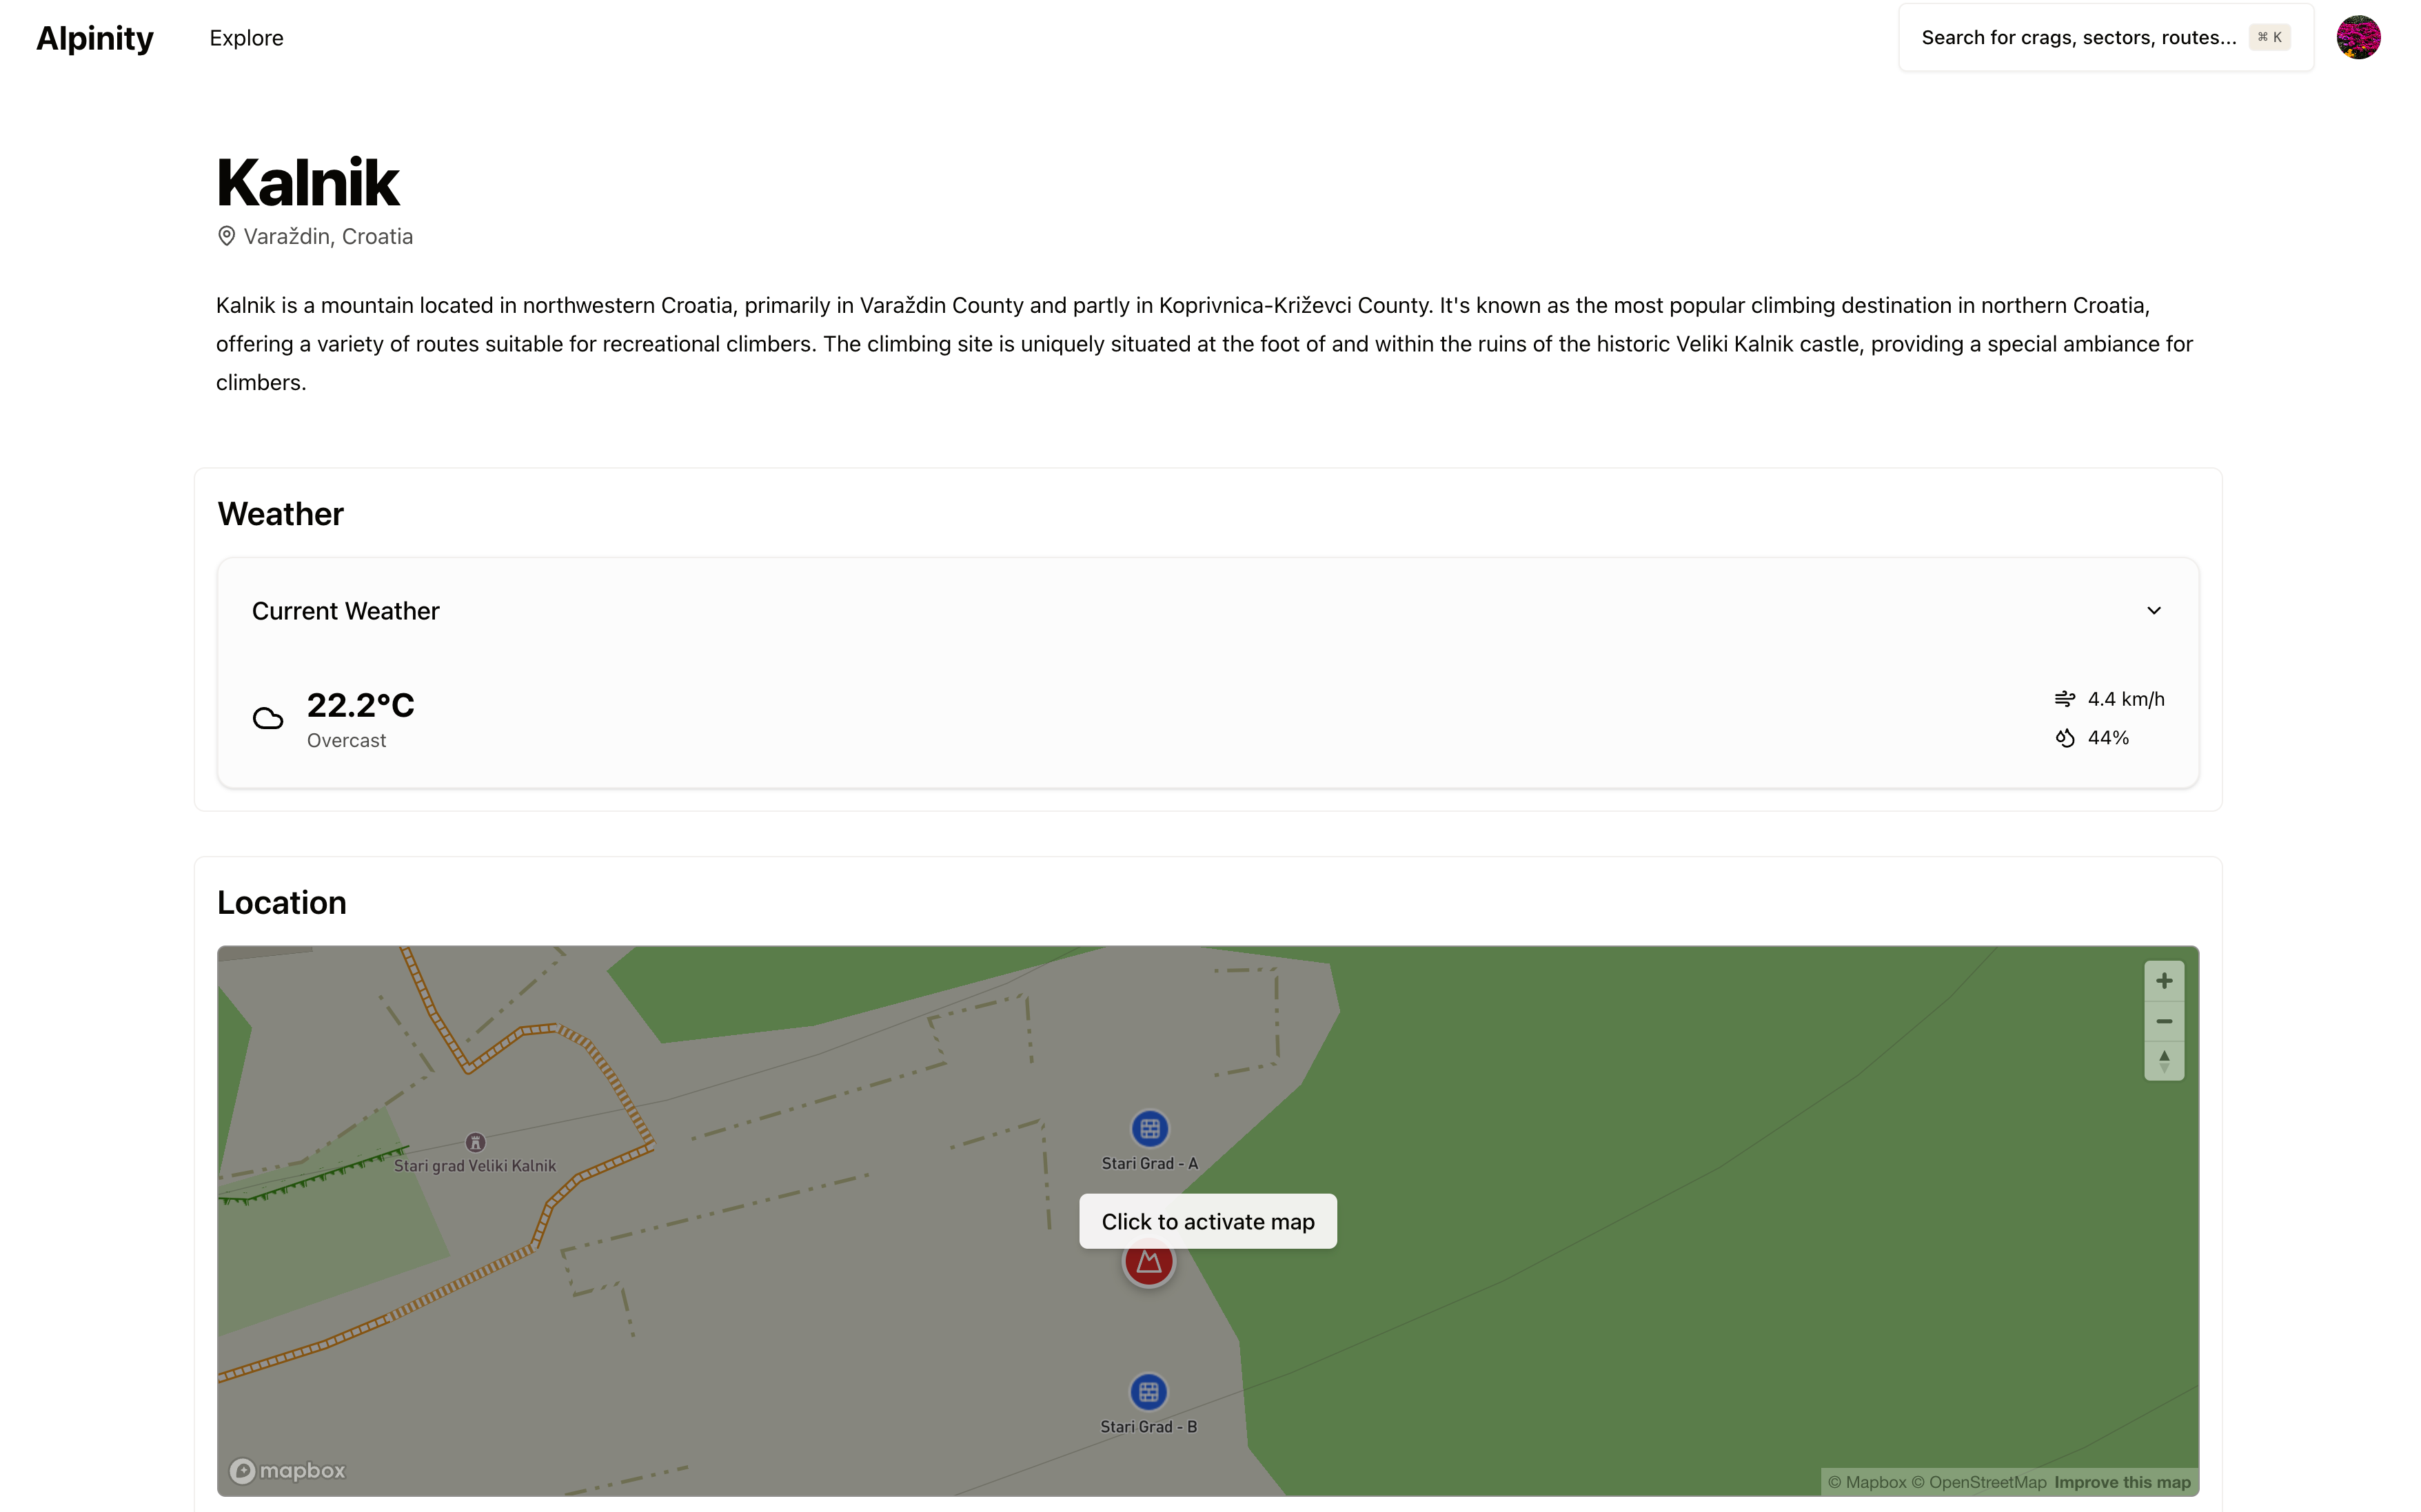
\includegraphics[width=0.9\textwidth]{images/implementacija/web/crag-details/crag-details-top.png}
        \caption{Web aplikacija}
        \label{fig:detalji_penjackih_lokacija_web}
    \end{subfigure}
    \caption{Detalji penjačke lokacije na mobilnoj i web aplikaciji}
    \label{fig:detalji_penjackih_lokacija_1}
\end{figure}

Odabirom penjačkih lokacija iz pretrage, s geografske karte ili drugih pregleda, korisnik pristupa zaslonu s detaljnim informacijama o penjačkoj lokaciji (slika~\ref{fig:detalji_penjackih_lokacija_1}). Zaslon je podijeljen na nekoliko cjelina. Na vrhu se nalazi istaknuta fotografija penjačkih lokacija, zajedno s nazivom penjačke lokacije i osnovnim podacima o broju sektora i penjačkih smjerova. 
Na web aplikaciji nalazi se isti prikaz, ali s manjim promjenama. Slika penjačke lokacije nalaze se ispod geografske karte, a broj sektora i penjačkih smjerova nalazi se u prikazu sektora i penjačkih smjerova.

\begin{figure}[H]
    \centering
    \begin{subfigure}[b]{\textwidth}
        \centering
        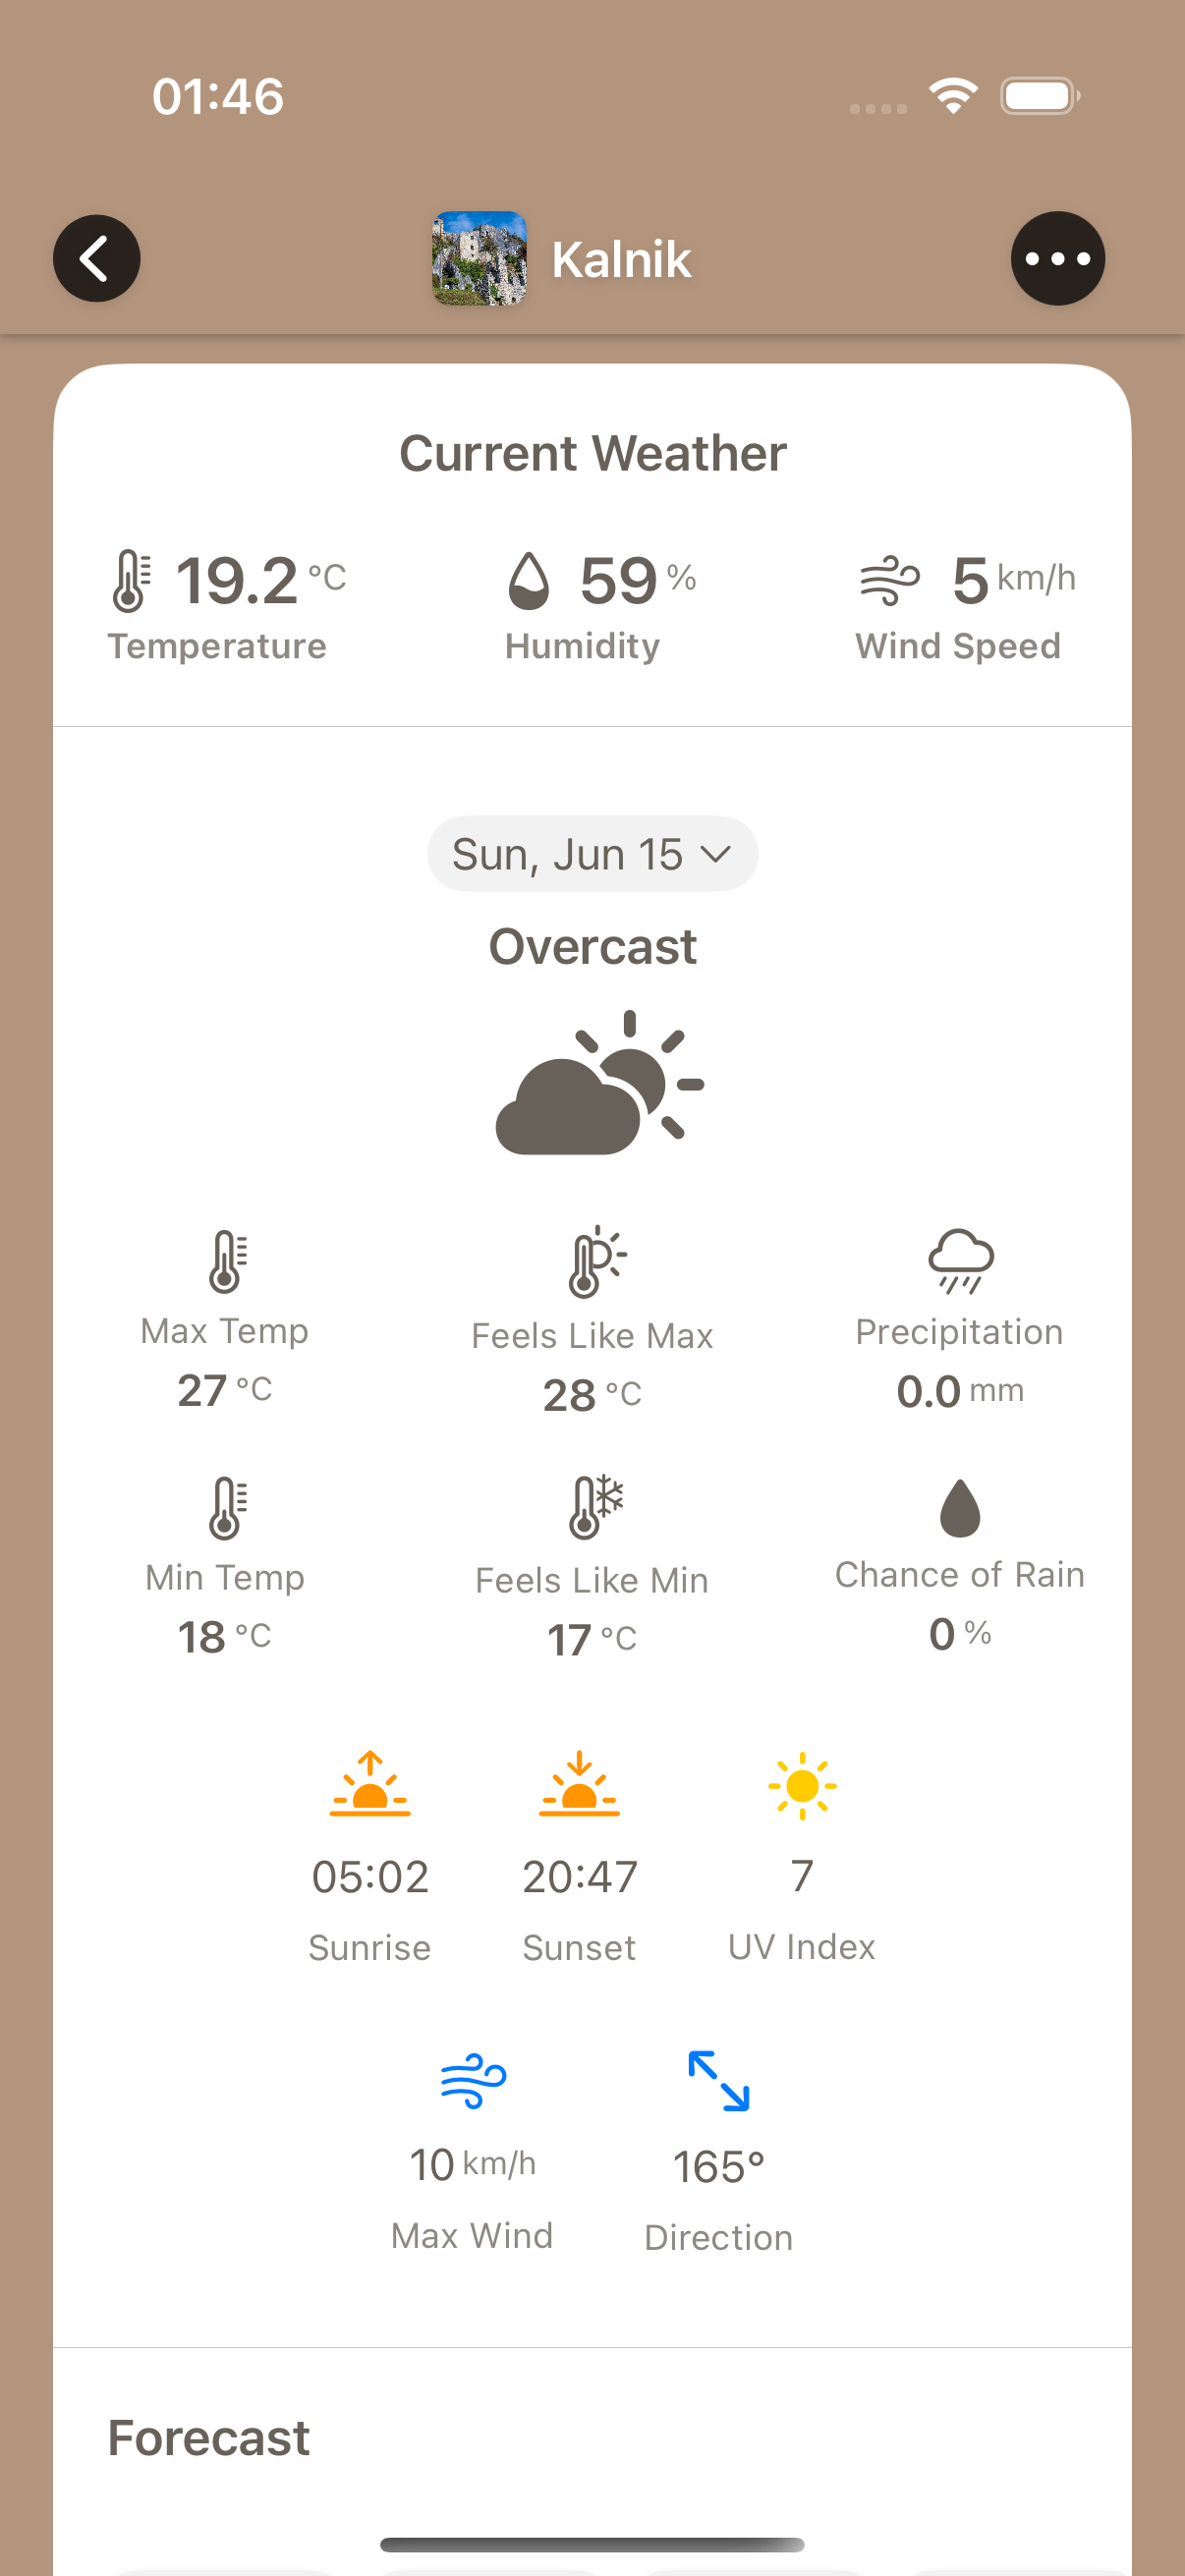
\includegraphics[width=0.35\textwidth]{images/implementacija/crag-details/crag-weather-1.png}
        \caption{Mobilna aplikacija}
        \label{fig:vremenska_prognoza_mob}
    \end{subfigure}
    \hfill
    \begin{subfigure}[b]{\textwidth}
        \centering
        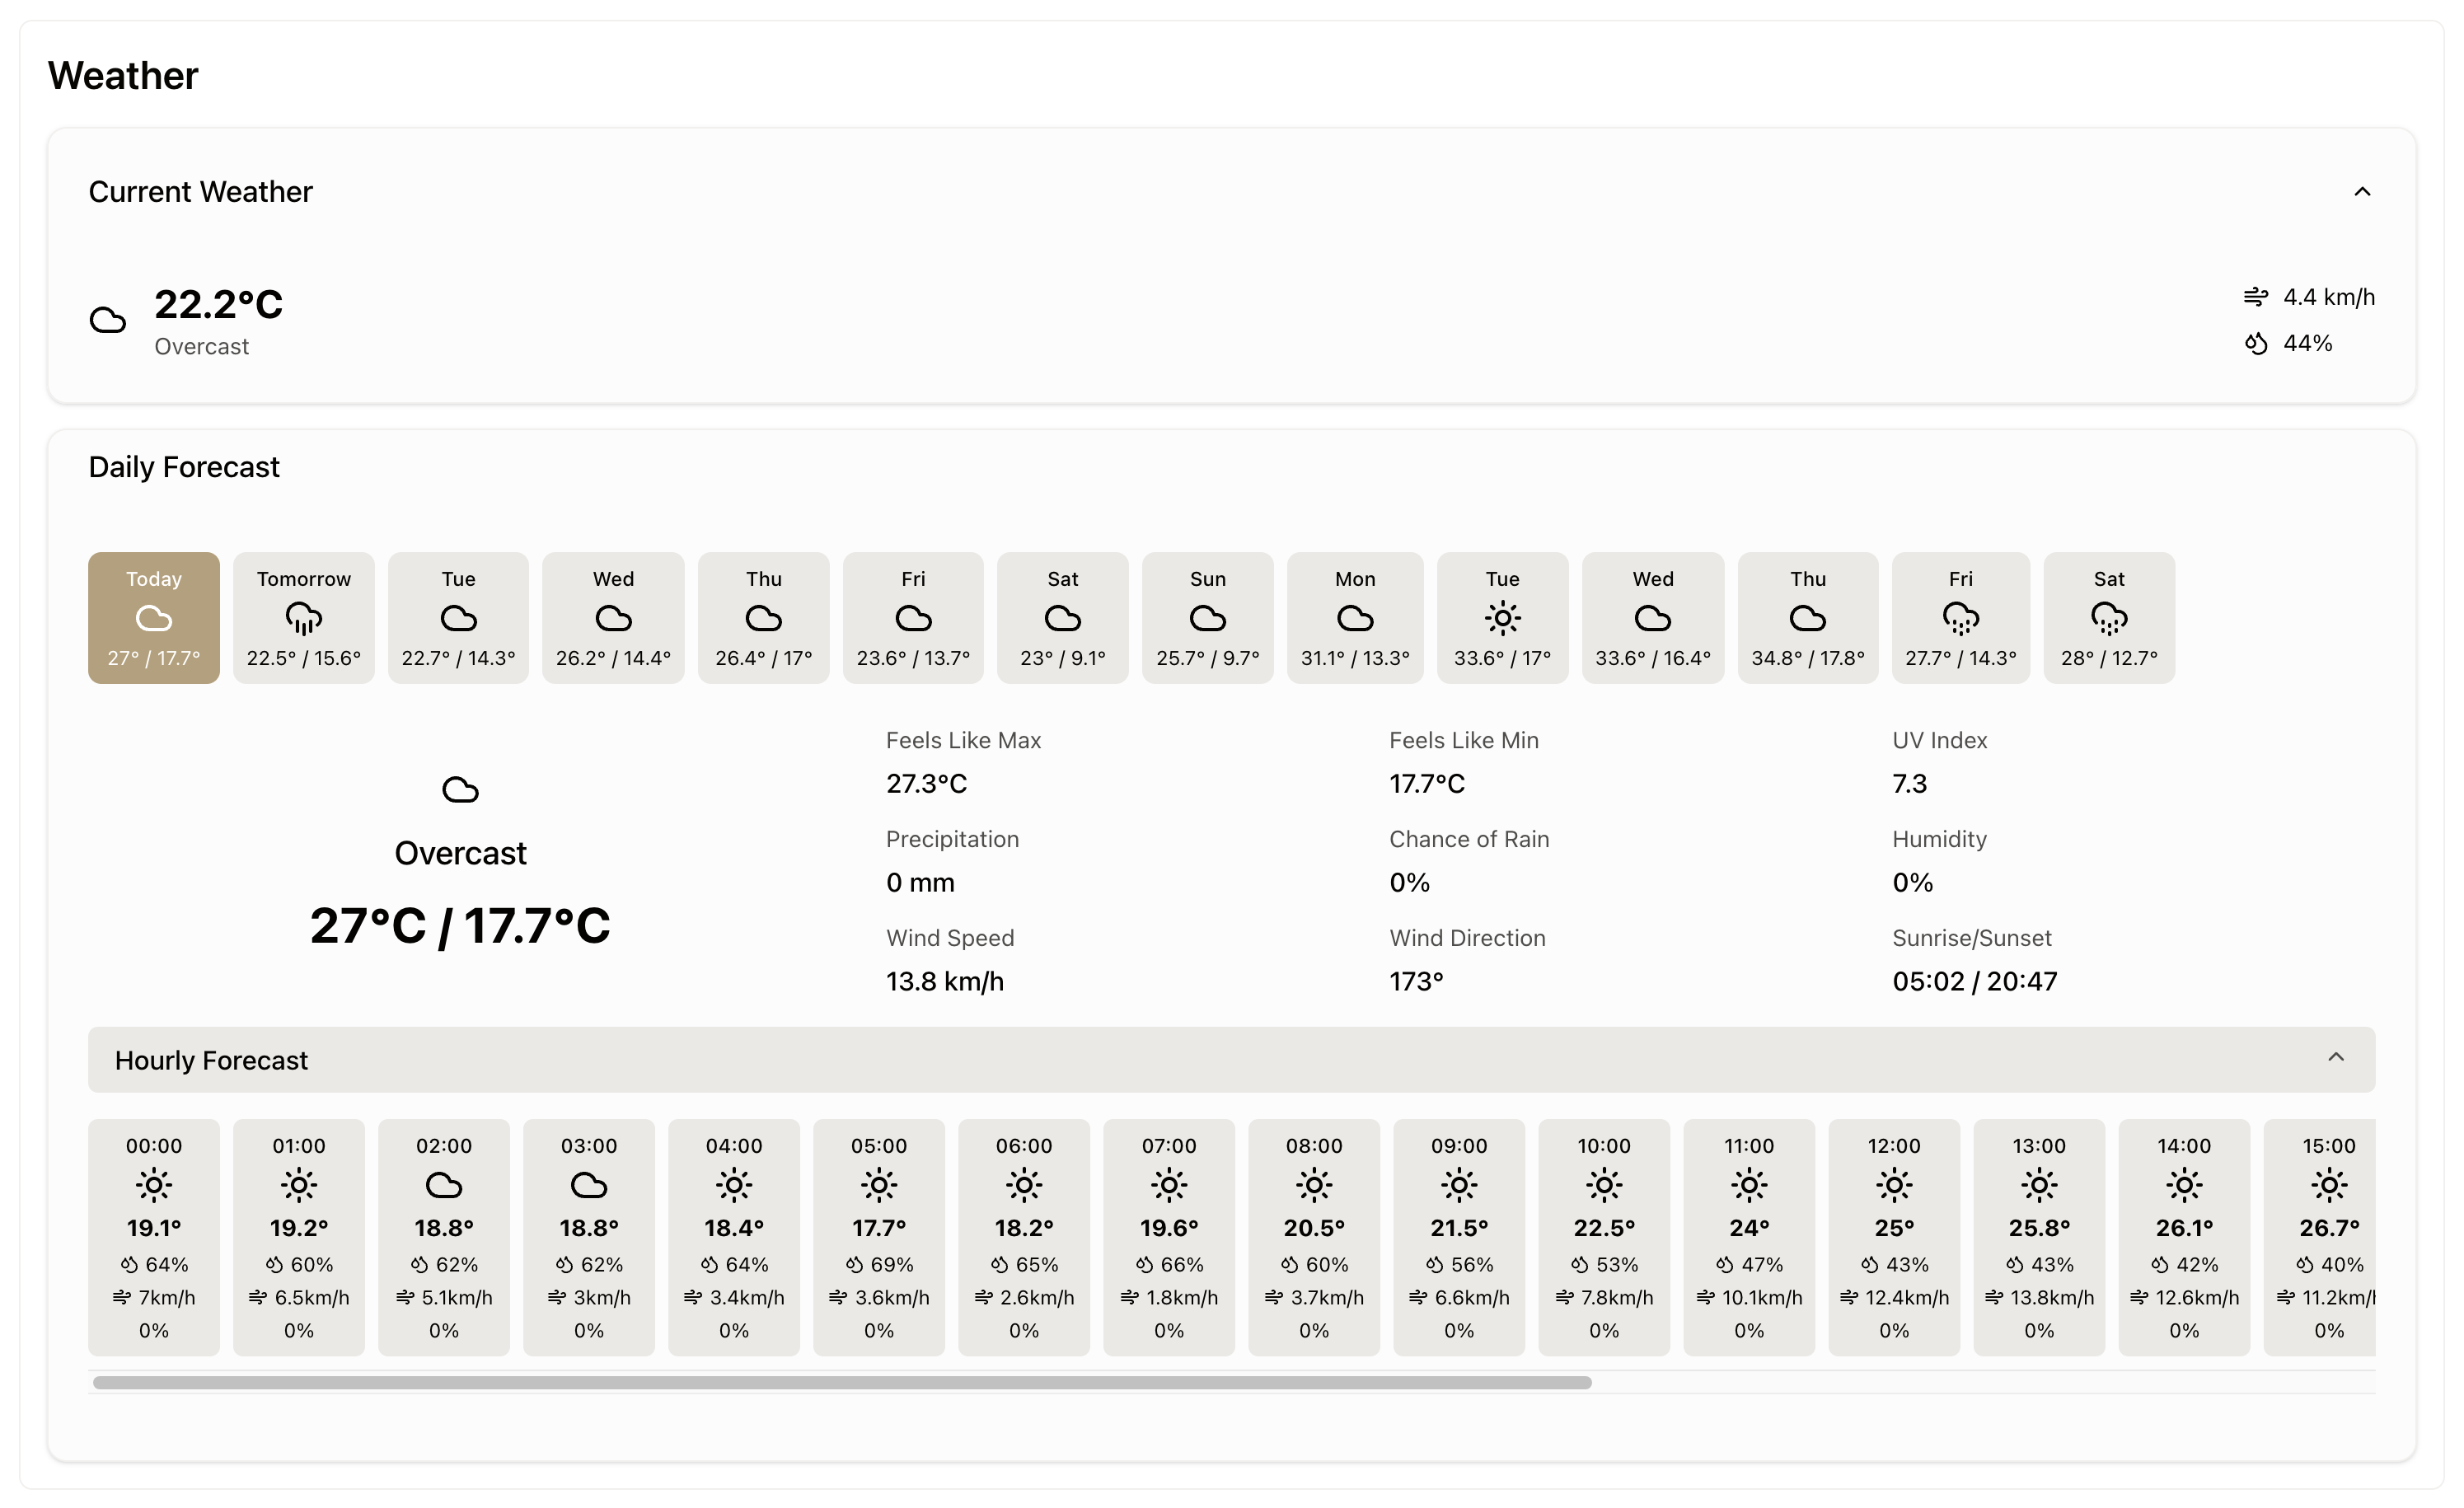
\includegraphics[width=0.9\textwidth]{images/implementacija/web/crag-details/crag-weather.png}
        \caption{Web aplikacija}
        \label{fig:vremenska_prognoza_web}
    \end{subfigure}
    \caption{Vremenska prognoza na mobilnoj i web aplikaciji}
    \label{fig:vremenska_prognoza}
\end{figure}

Odmah ispod, nalazi se komponenta s vremenskom prognozom (slika~\ref{fig:vremenska_prognoza}). Ona prikazuje trenutne vremenske uvjete, kao i detaljnu prognozu po satima za sljedećih 14 dana. Detaljna prognoza uključuje temperaturu, vjerojatnost i količina padalina, brzinu vjetra, UV indeks i ostale relevantne podatke. Ova funkcionalnost je važna za planiranje penjačkih izleta.


Nakon komponente vremenske prognoze sljedi interaktivna karta penjačkih lokacija koja prikazuje precizne lokacije svih sektora, omogućujući korisniku lako snalaženje i planiranje kretanja između njih (slika~\ref{fig:interaktivna_karta}). 

\begin{figure}[H]
    \centering
    \begin{subfigure}[b]{\textwidth}
        \centering
        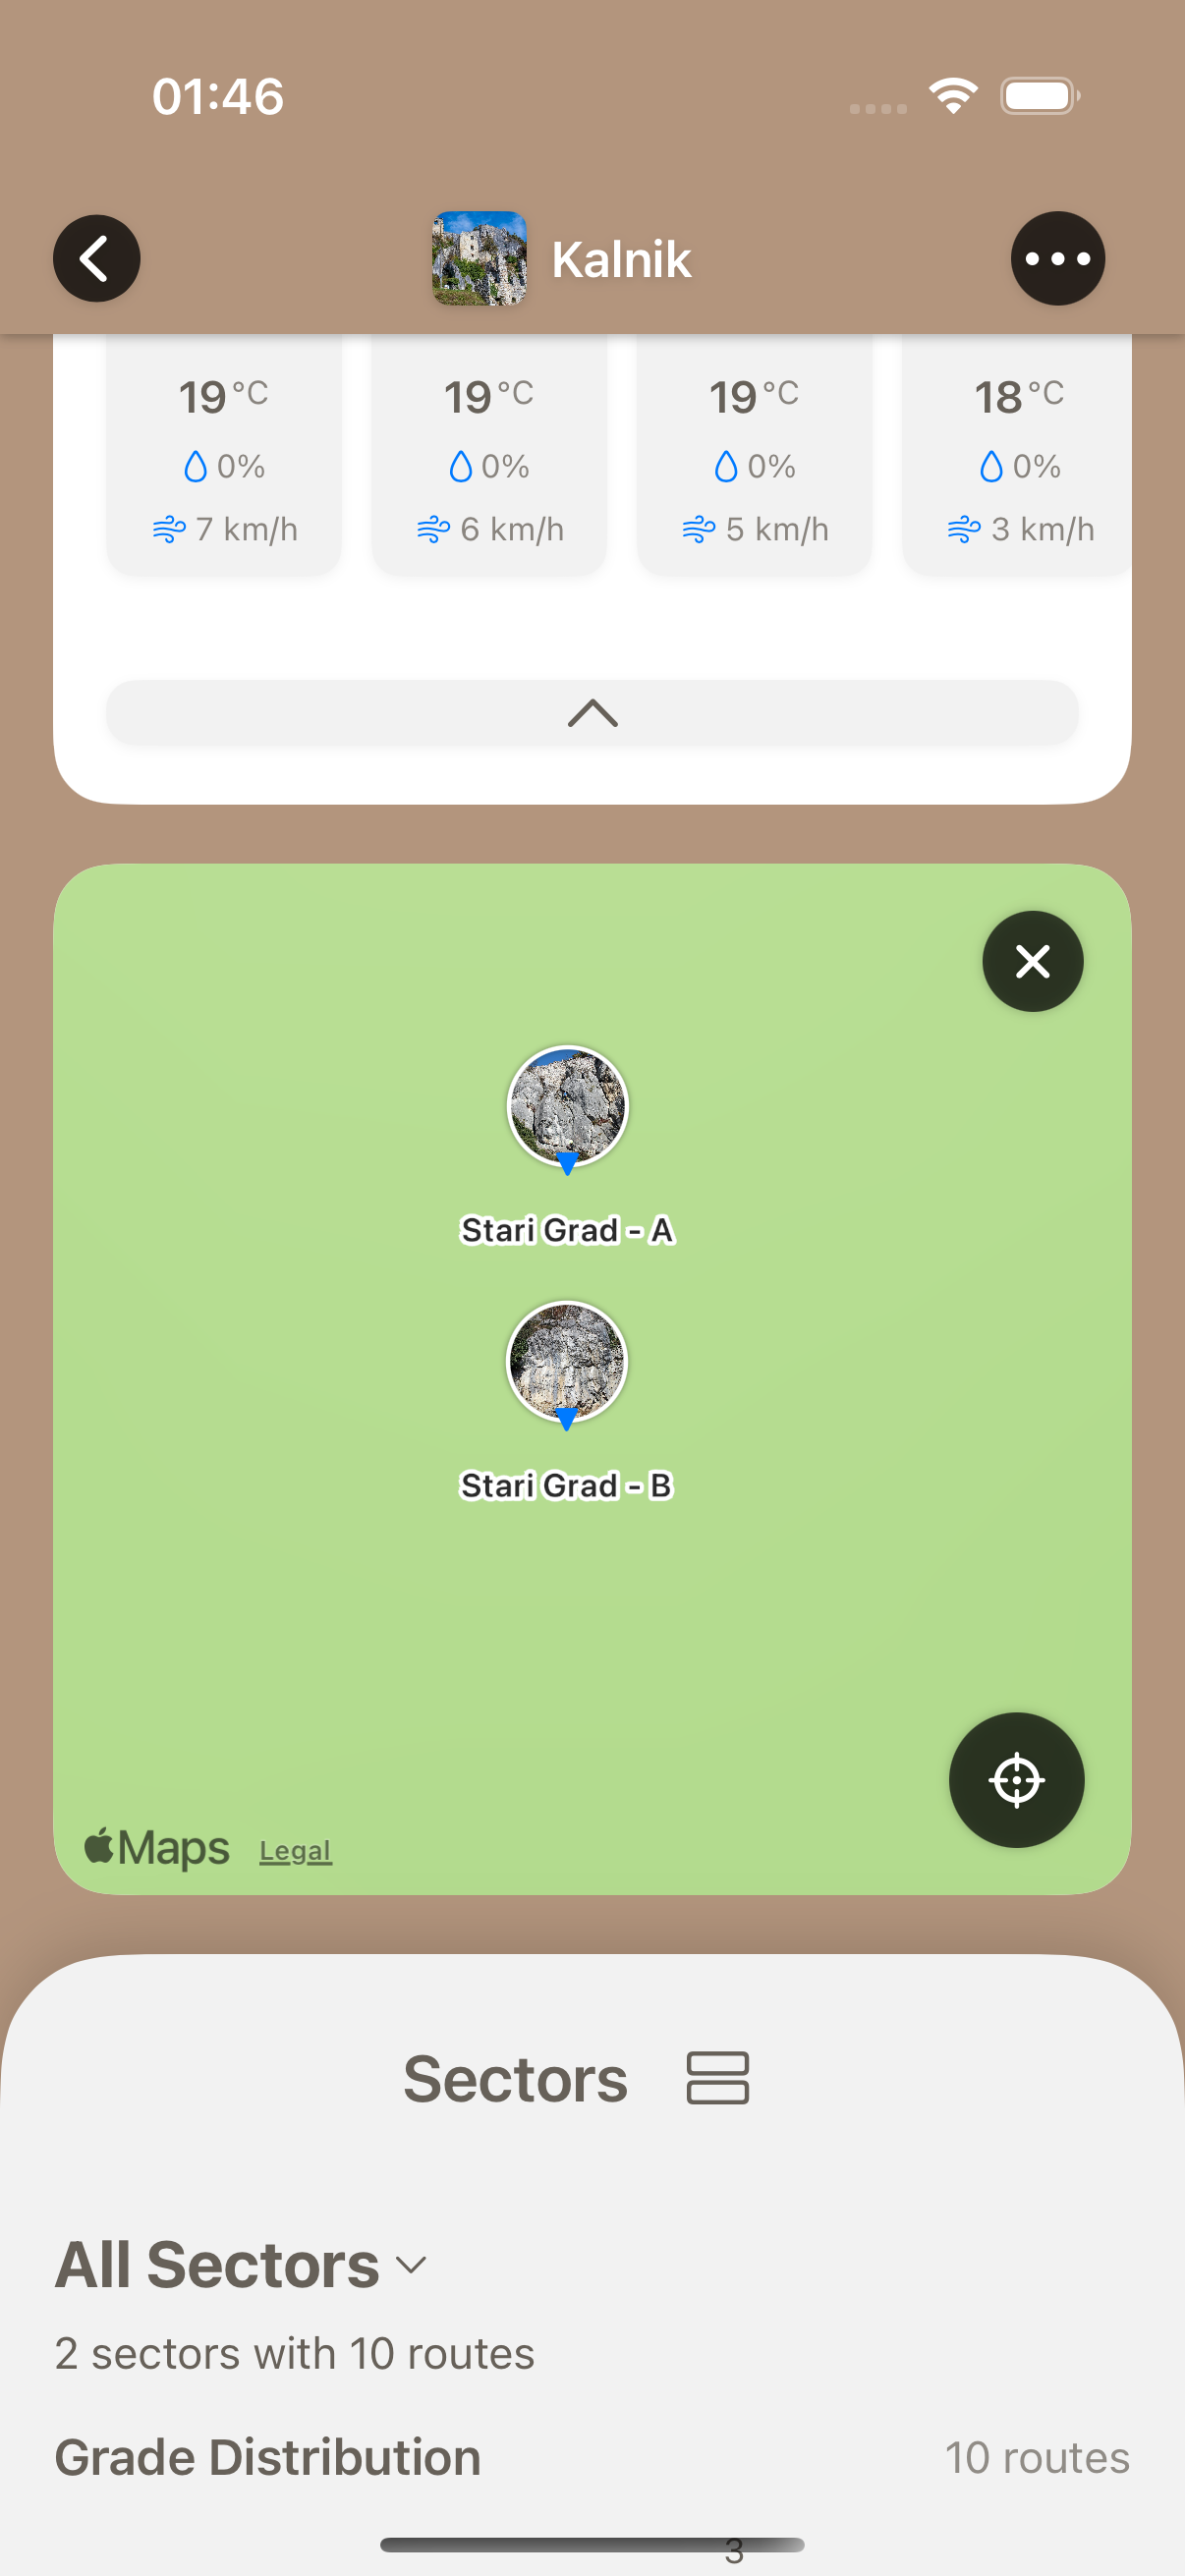
\includegraphics[width=0.35\textwidth]{images/implementacija/crag-details/crag-map.png}
        \caption{Mobilna aplikacija}
        \label{fig:interaktivna_karta_mob}
    \end{subfigure}
    \hfill
    \begin{subfigure}[b]{\textwidth}
        \centering
        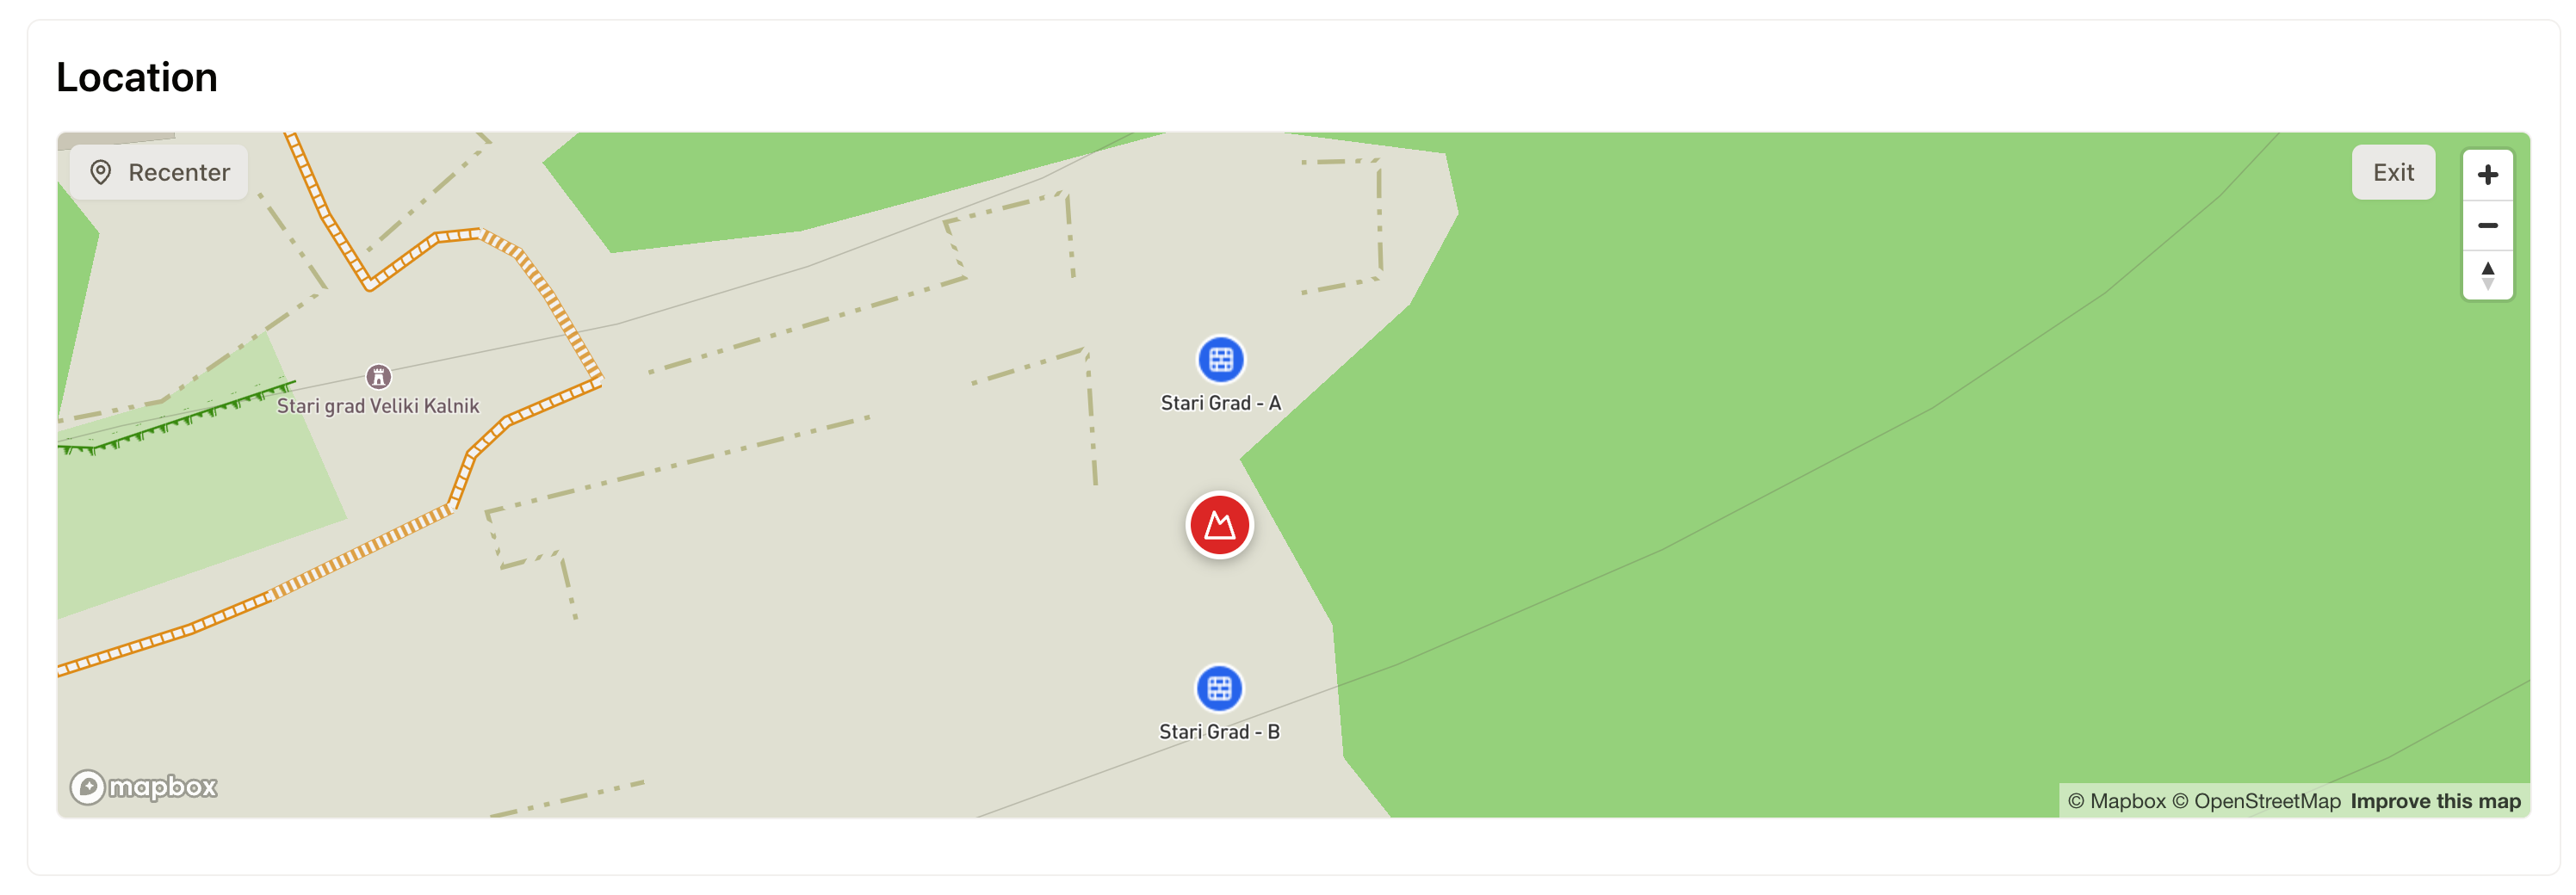
\includegraphics[width=0.9\textwidth]{images/implementacija/web/crag-details/crag-map.png}
        \caption{Web aplikacija}
        \label{fig:interaktivna_karta_web}
    \end{subfigure}
    \caption{Interaktivna karta penjačkih lokacija}
    \label{fig:interaktivna_karta}
\end{figure}

Ispod karte nalazi se prikaz detalja za sektore. Prije ikakvih odabira, korisniku se prikazuje popis svih penjačkih smjerova grupiranih po sektorima te distribucija težina na penjačkoj lokaciji (slika~\ref{fig:prikaz_detalja_za_sektore}). 

\begin{figure}[H]
    \centering
    \begin{subfigure}[b]{0.4\textwidth}
        \centering
        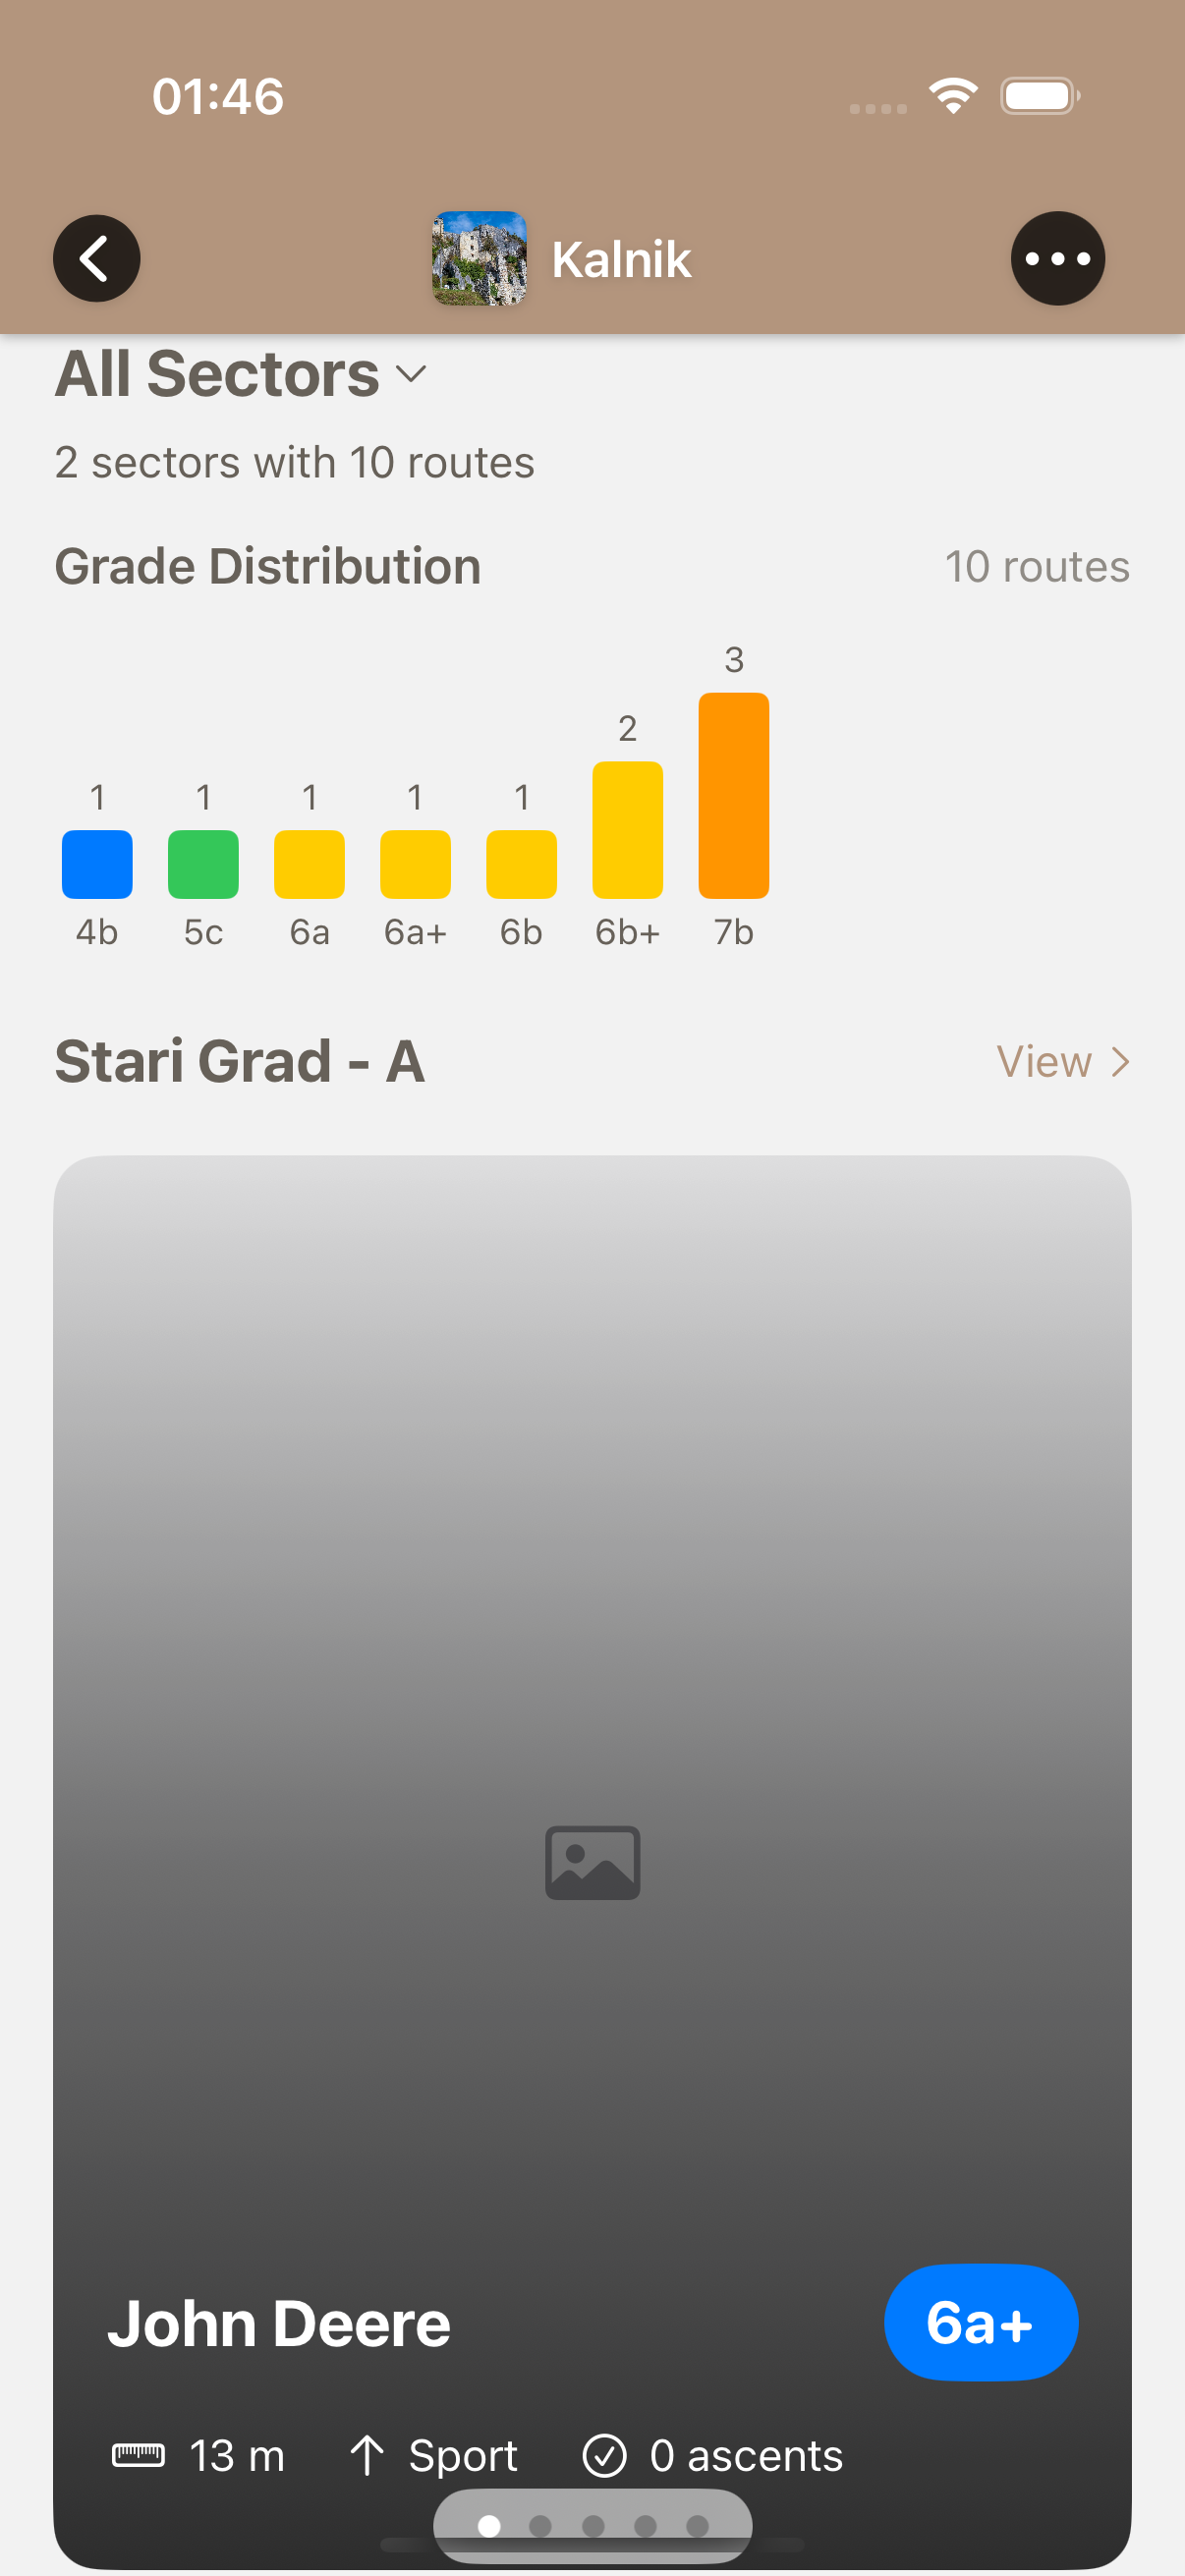
\includegraphics[width=0.7\textwidth]{images/implementacija/crag-details/crag-all-sectors-tabs.png}
        \caption{Mobilna aplikacija}
        \label{fig:prikaz_detalja_za_sektore_mob}
    \end{subfigure}
    \hfill
    \begin{subfigure}[b]{0.55\textwidth}
        \centering
        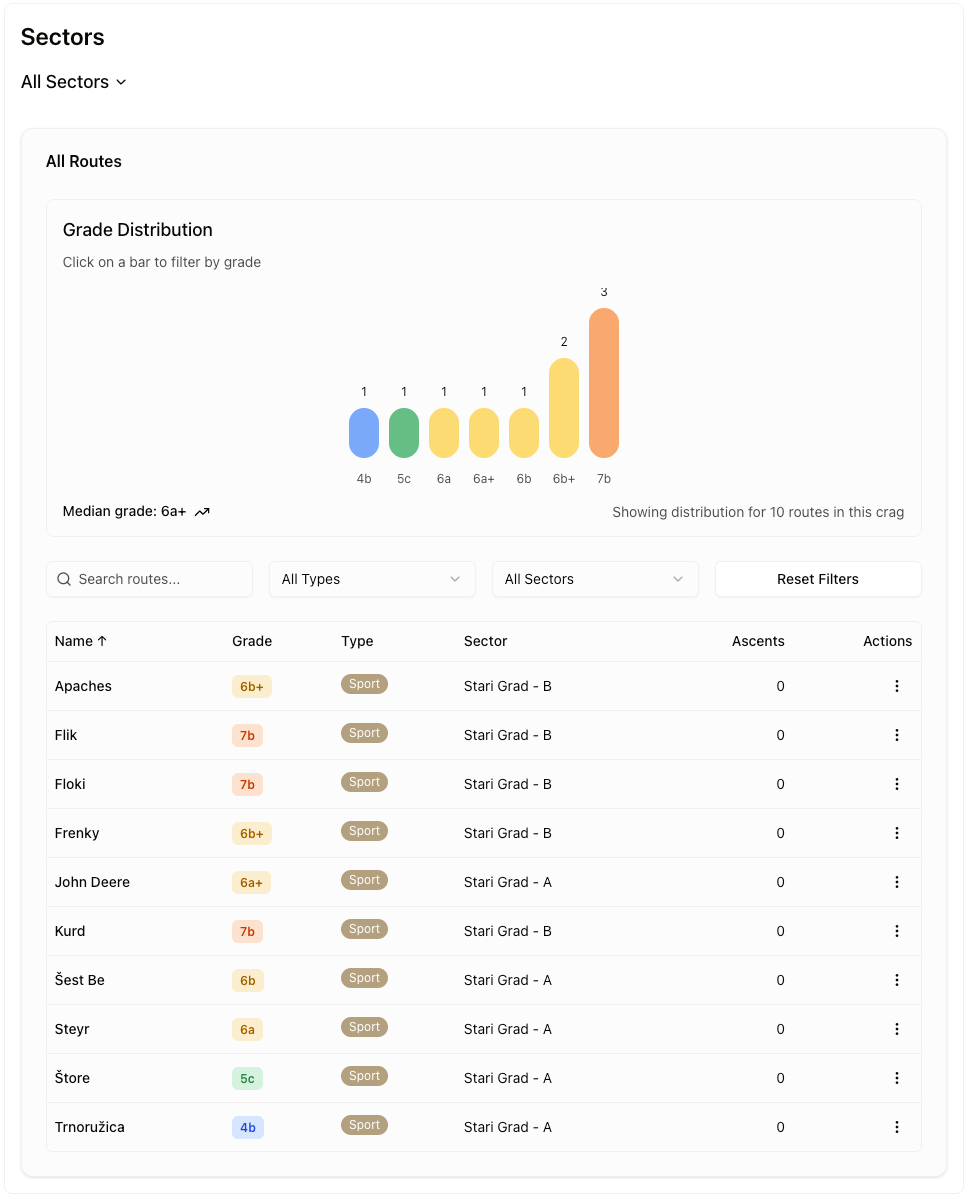
\includegraphics[width=1\textwidth]{images/implementacija/web/crag-details/crag-all-sectors.png}
        \caption{Web aplikacija}
        \label{fig:prikaz_detalja_za_sektore_web}
    \end{subfigure}
    \caption{Prikaz detalja za sektore}
    \label{fig:prikaz_detalja_za_sektore}
\end{figure}

Klikom na određenu težinu u grafu filtriraju se svi penjački smjerovi koji pripadaju odabranoj težini. Lista penjačkih smjerova na mobilnoj aplikaciji je horizontalna lista koja prikazuje penjački smjer u većem formatu kako bi se mogla bolje vidjeti slika penjačkog smjera. Preko slike nalaze se detalji o penjačkom smjeru poput naziva, težine, dužine, tipa i broja uspona.

\begin{figure}[H]
    \centering
    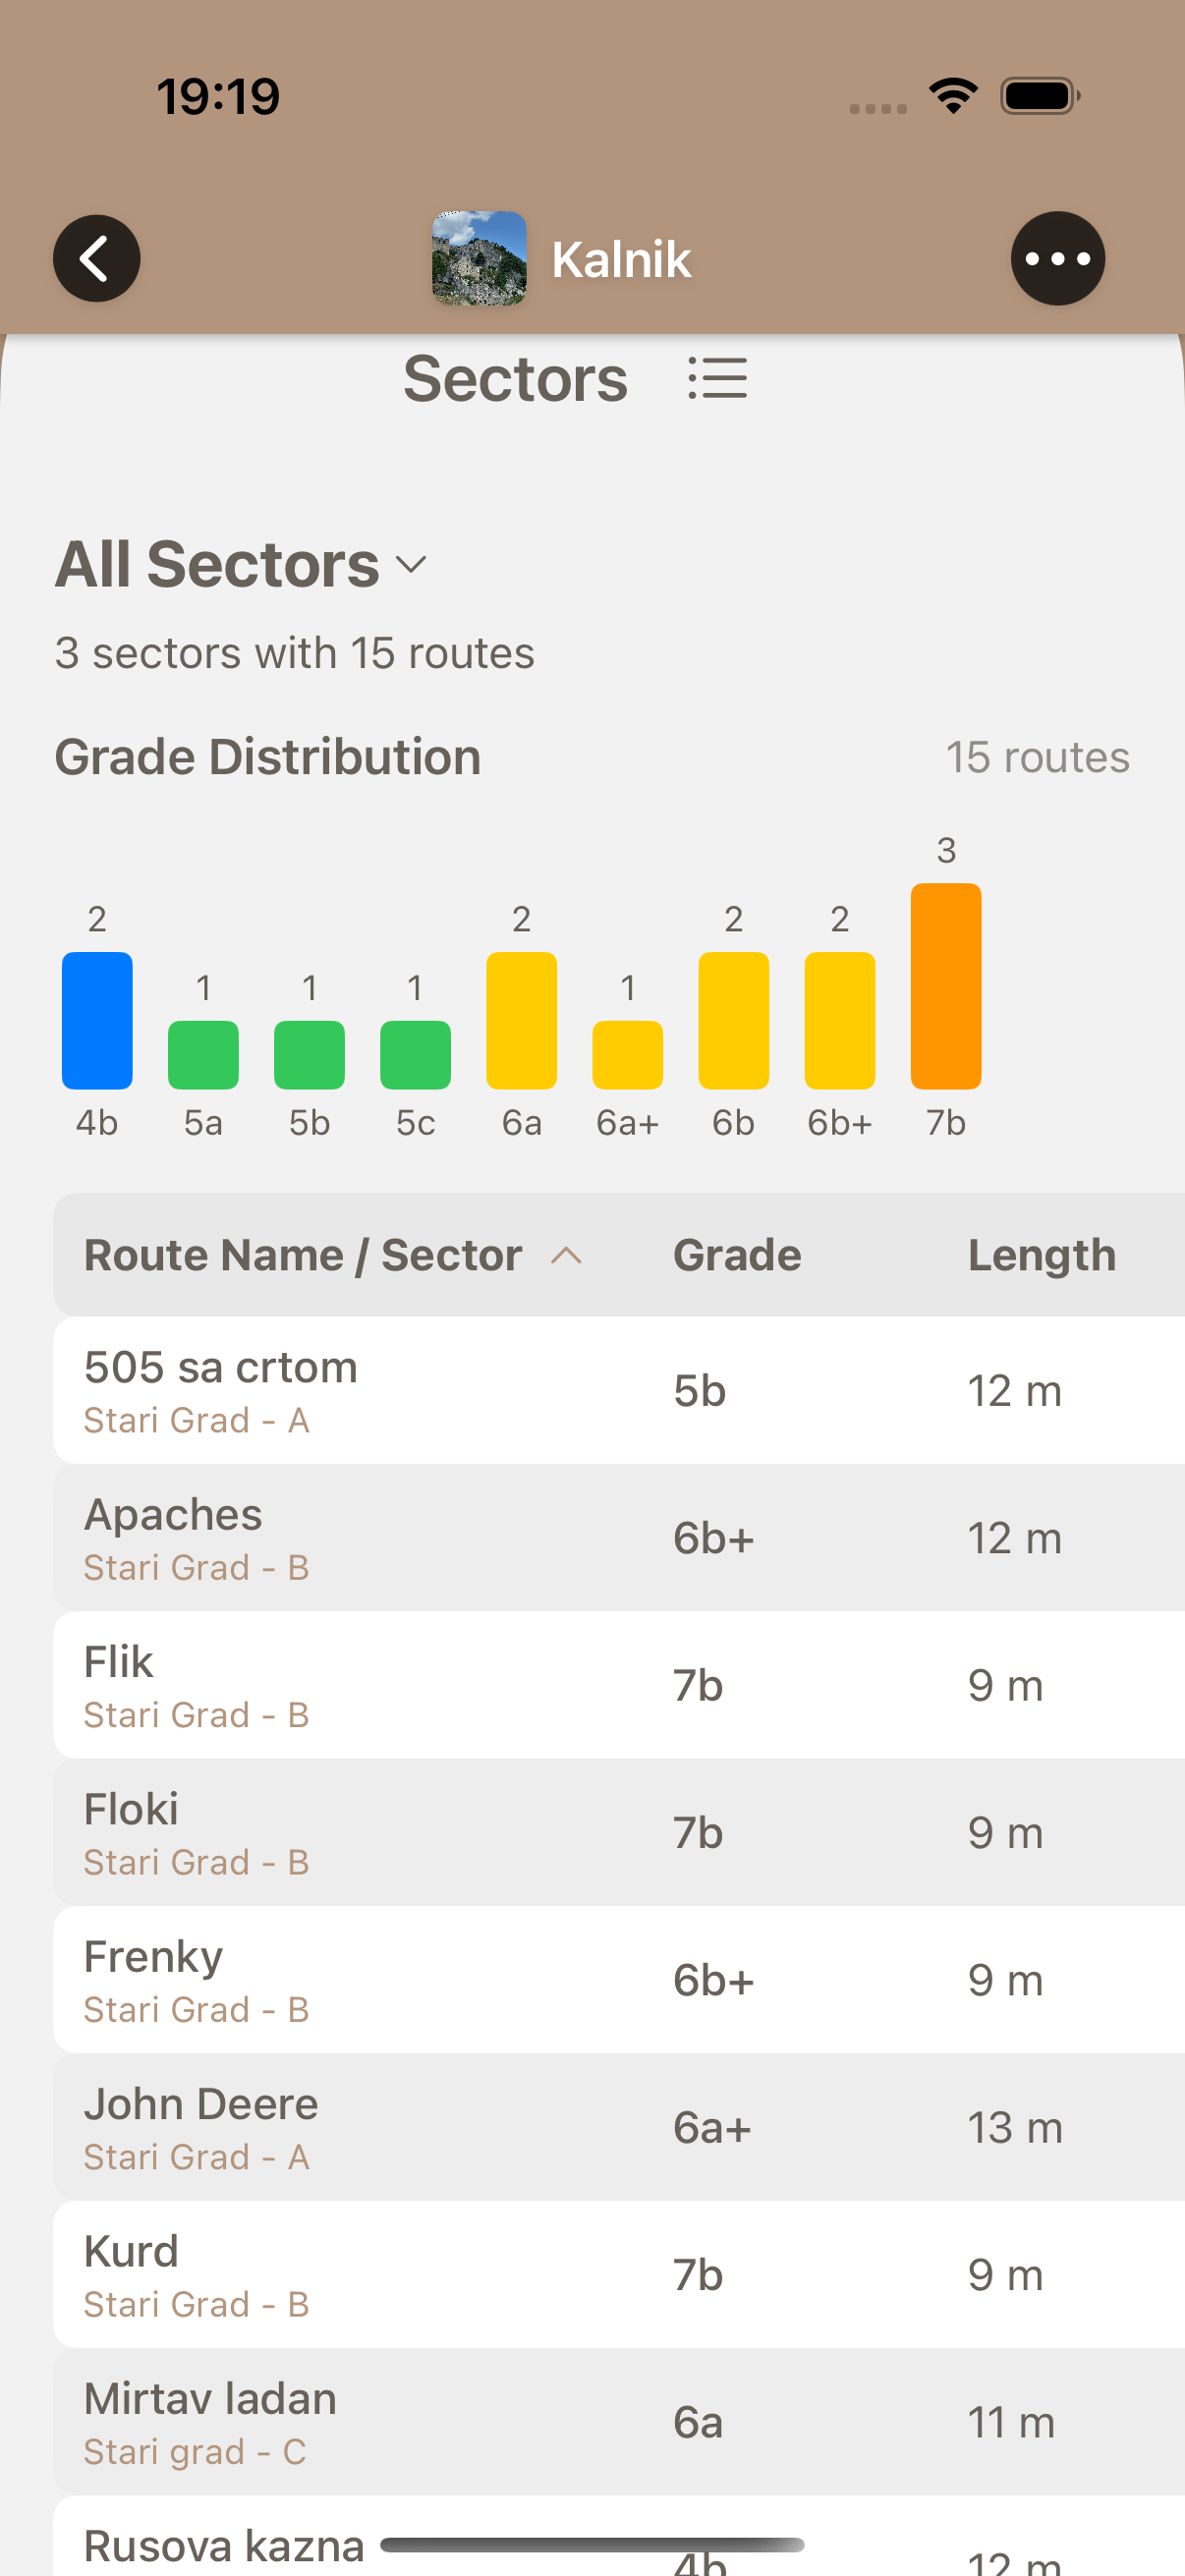
\includegraphics[width=0.35\textwidth]{images/implementacija/crag-details/crag-all-sectors-table.png}
    \caption{Tablični prikaz sektora na mobilnoj aplikaciji}
    \label{fig:tablični_prikaz_sektora}
\end{figure}

Ako korisnik preferira tablični prikaz na mobilnoj aplikaciji, može to promijeniti klikom na gumb pored naslova "Sektori" (eng. \textit{Sectors}) (slika~\ref{fig:tablični_prikaz_sektora}). Na web aplikaciji tablični prikaz je zadani prikaz. Tablični prikaz omogućuje pregled svih penjačkih smjerova te sortiranje po nazivu, težini, dužini, tipu te broju uspona. S obzirom da na web aplikaciji nije grupiran prikaz po sektorima, postoje filteri koji korisnik može koristiti za filtriranje penjačkih smjerova po imenu, tipu i sektoru.

Klikom na izbornik "Svi sektori" (eng. \textit{All sectors}) korisniku prikazuje se popis svih sektora na penjačkoj lokaciji (slika~\ref{fig:prikaz_detalja_za_odabrani_sektor}). 

\begin{figure}[H]
    \centering
    \begin{subfigure}[b]{0.35\textwidth}
        \centering
        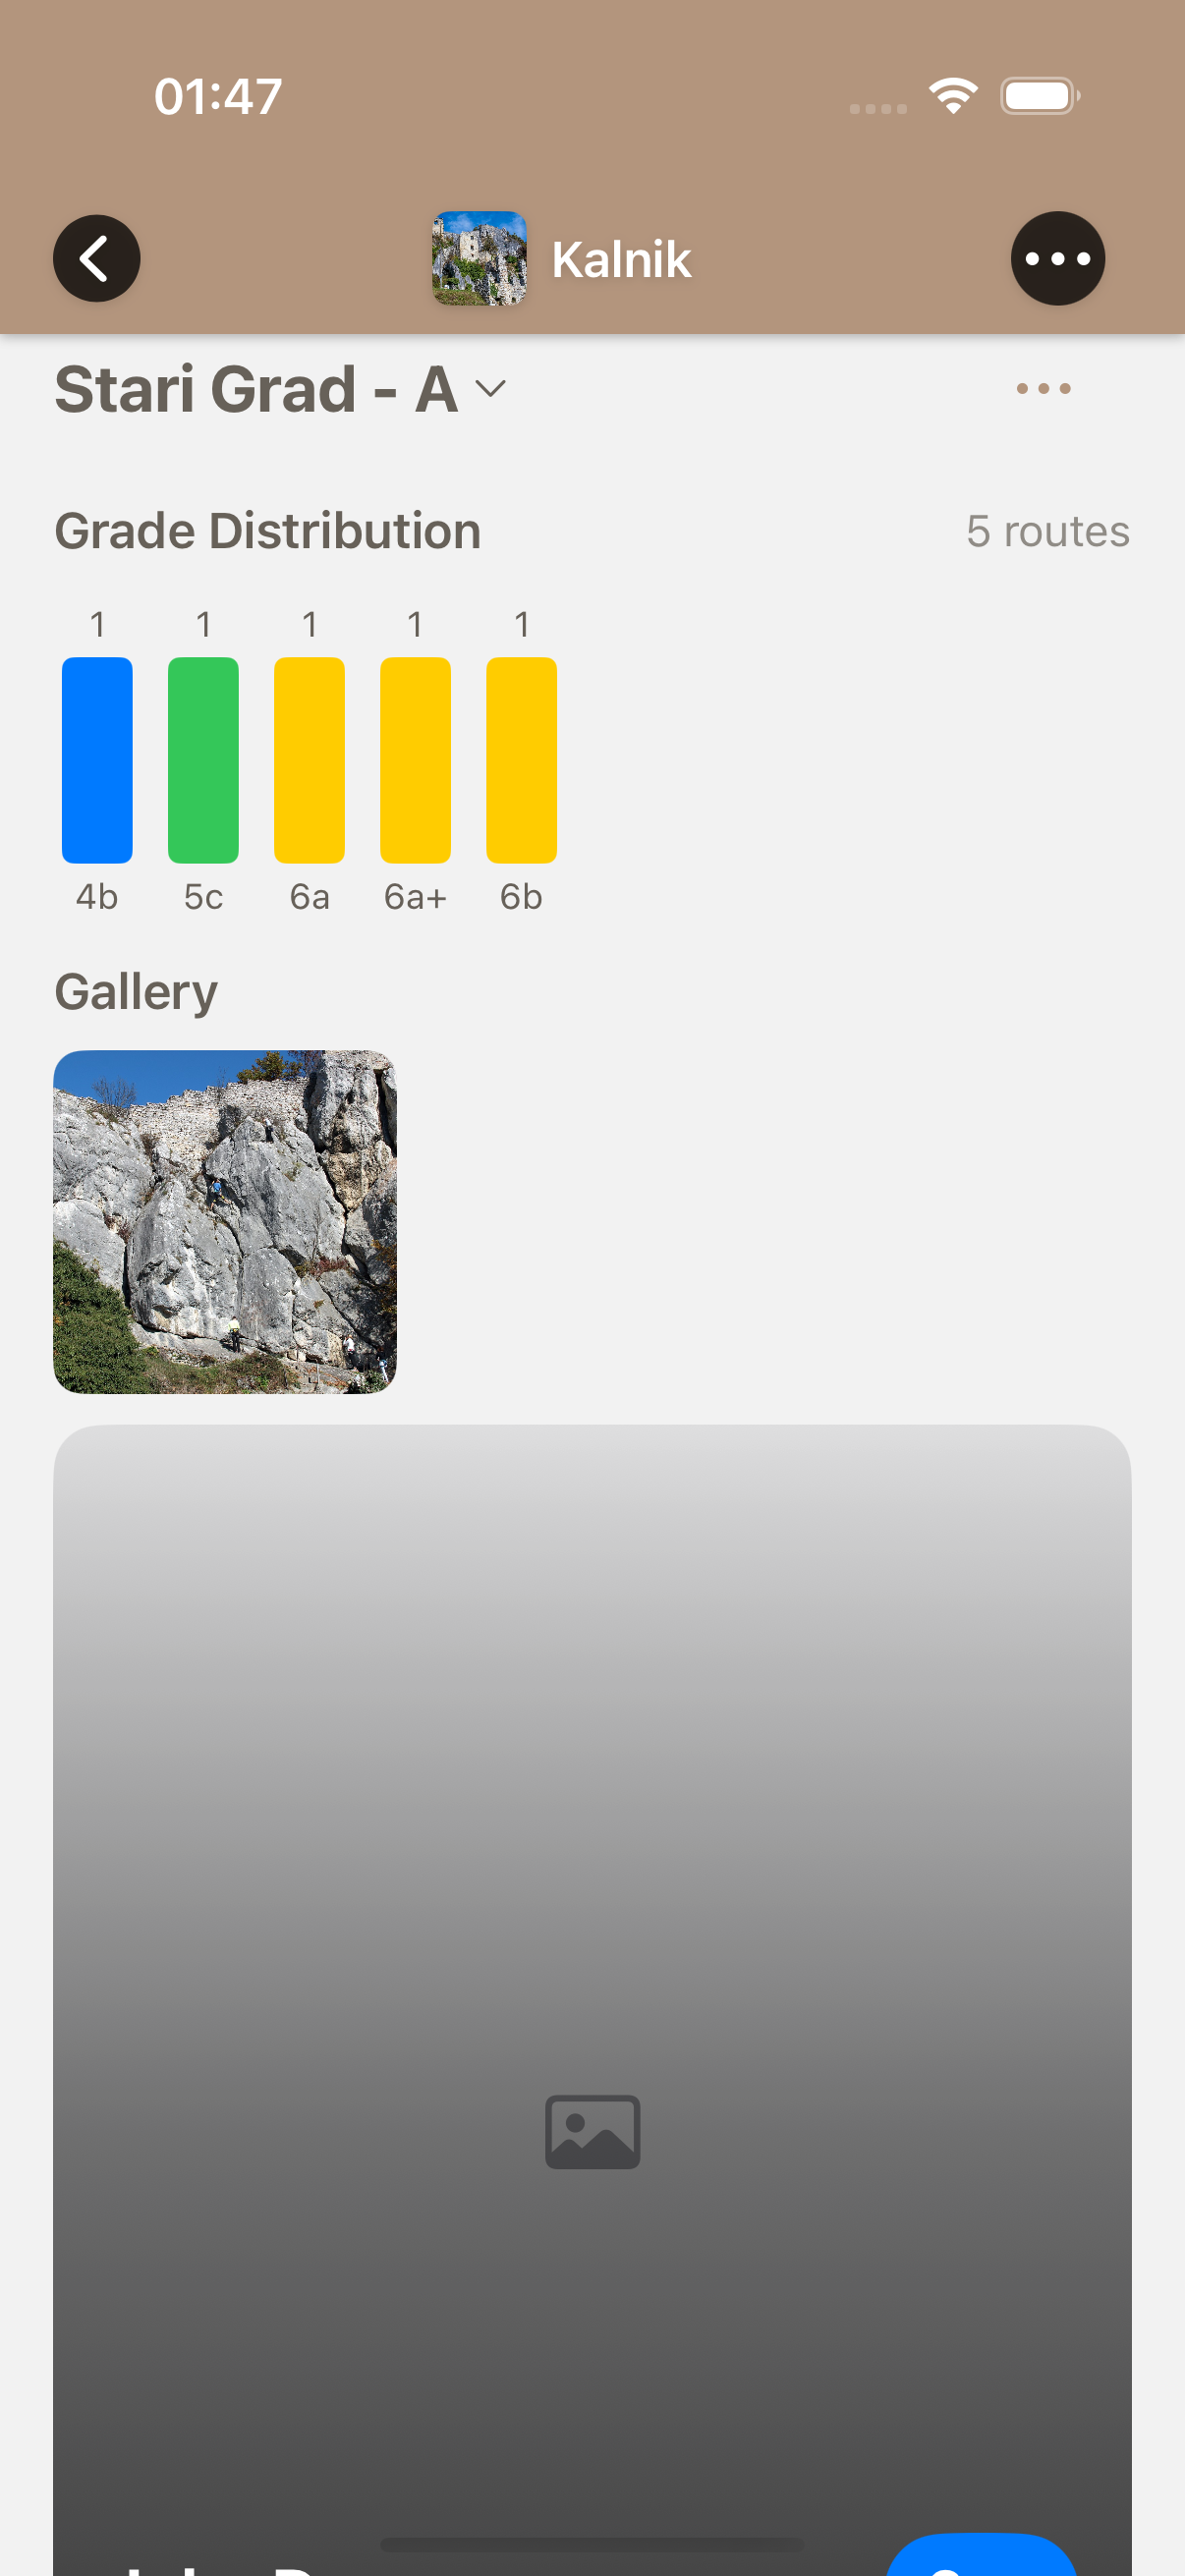
\includegraphics[width=\textwidth]{images/implementacija/crag-details/crag-selected-sector.png}
        \caption{Mobilna aplikacija}
        \label{fig:prikaz_detalja_za_odabrani_sektor_mob}
    \end{subfigure}
    \hfill
    \begin{subfigure}[b]{0.6\textwidth}
        \centering
        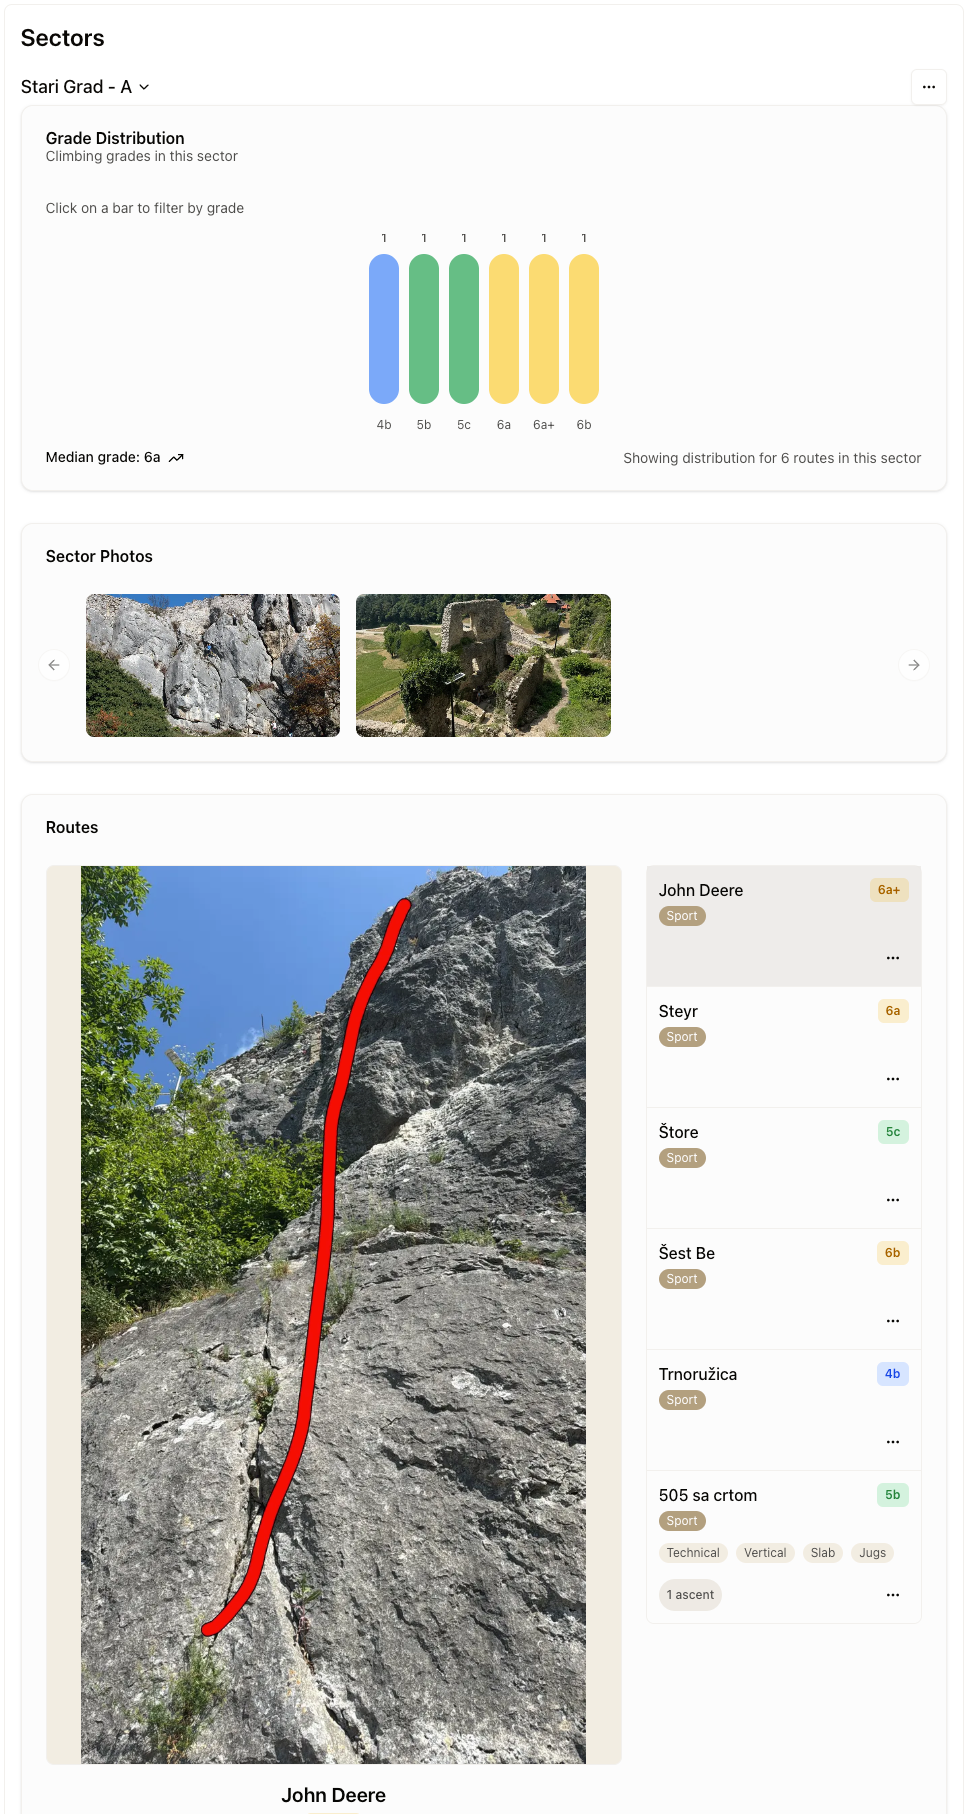
\includegraphics[width=1\textwidth]{images/implementacija/web/crag-details/crag-selected-sector.png}
        \caption{Web aplikacija}
        \label{fig:prikaz_detalja_za_odabrani_sektor_web}
    \end{subfigure}
    \caption{Prikaz detalja za odabrani sektor}
    \label{fig:prikaz_detalja_za_odabrani_sektor}
\end{figure}

Odabirom određenog sektora, korisniku se prikazuje graf težina filtriran po odabranom sektoru, slike sektora te popis svih penjačkih smjerova u tom sektoru. Klikom na određeni stupac na grafu težina, popis penjačkih smjerova se filtrira po označenoj težini. Tablični prikaz je isto dostupan klikom na gumb pored naslova "Sektori" (eng. \textit{Sectors}). Na web aplikaciji nalaze se ista funkcionalnost, ali s različitim prikazom.



